\documentclass[11pt]{article}
\usepackage{setspace}
\setstretch{0.8}  % 调整为合适的行距倍数
\setlength{\textfloatsep}{1pt}
\setlength{\intextsep}{1pt}
\usepackage{times} % Times New Roman font
\usepackage{graphicx} % For images
\usepackage{enumitem} % For numbered items
\usepackage{lipsum} % For dummy text
\usepackage{hyperref} % For references
\hypersetup{
colorlinks=true,
linkcolor=blue,
filecolor=magenta,
urlcolor=cyan,
} % For hyperlinks
\usepackage{amsmath} % For math equations
\usepackage{cleveref} % For clever references
\crefname{appendix}{Appendix}{Appendices}
\usepackage{fancyvrb} % For code display
\usepackage{fancyhdr} % For custom headers
\usepackage{pythonhighlight} % For Python code
\usepackage{float} % For image positioning
\usepackage{amsmath} % For math equations
\usepackage{xcolor} % For custom colors
\usepackage{natbib} % For bibliography
\usepackage{appendix} % For appendices
\usepackage[font={small,it}]{caption}
% \usepackage{mwe}% For custom captions
\usepackage{listings}
\usepackage{color}
\usepackage{amsmath}
\usepackage{graphicx}
\usepackage{hyperref}
\usepackage{geometry}
\usepackage{caption}
\captionsetup{font={small}}
\usepackage{ctex}
\usepackage{siunitx}
\usepackage{booktabs}
\renewcommand{\tablename}{Table}
\renewcommand{\figurename}{Figure}
\renewcommand{\abstractname}{Abstract}
\geometry{a4paper, margin=1in}
\definecolor{codegreen}{rgb}{0,0.6,0}
\definecolor{codegray}{rgb}{0.5,0.5,0.5}
\definecolor{codepurple}{rgb}{0.58,0,0.82}
\definecolor{backcolour}{rgb}{0.95,0.95,0.92}
\usepackage{fancyhdr}
\setlength{\headheight}{13.59999pt}
\addtolength{\topmargin}{-1.59999pt}
\lstdefinestyle{mystyle}{
backgroundcolor=\color{backcolour},
commentstyle=\color{codegreen},
keywordstyle=\color{magenta},
numberstyle=\tiny\color{codegray},
stringstyle=\color{codepurple},
basicstyle=\ttfamily\footnotesize,
breakatwhitespace=false,
breaklines=true,
captionpos=b,
keepspaces=true,
numbers=left,
numbersep=5pt,
showspaces=false,
showstringspaces=false,
showtabs=false,
tabsize=2
}
\lstset{style=mystyle}
\lstnewenvironment{outputlisting}{
\lstset{
basicstyle=\ttfamily\footnotesize,
frame=single,
backgroundcolor=\color{lightgray},
keywordstyle=\color{blue},
breaklines=true,
postbreak=\mbox{\textcolor{red}{$\hookrightarrow$}\space},
xleftmargin=.1\textwidth,
xrightmargin=.1\textwidth,
captionpos=b,
language=[Sharp]C,
numbers=none,
tabsize=2,
showstringspaces=false
}
}{}

\title{Complex Network Analysis of Classical Chinese Literature: Insights from the Confucian Canon of Scripta Sinica Corpus}
\author{Yichi Zhang u7748799}
\date{May, 2024}

\begin{document}
\setstretch{1.0}
\maketitle

\begin{abstract}
    The study of language as a complex system has attracted a lot of attention recently due to the quick development and widespread use of NLP and LLM recently. Network science offers a strong framework for detecting the structure of linguistic systems. Chinese, one of the most significant and unique languages in the world, has been studied by numerous academics. Nonetheless, while being the ancestor of Modern Chinese, Classical Chinese has received little attention, most likely because of corpus limitations. In this project, we investigate the topological characteristics of Classical Chinese literature using complex network analysis, concentrating on Scripta Sinica corpus. Through the construction of two distinct network types from the corpus, a Character Co-occurrence Network (CCN) and a Character-Sentence Network (CSN), we reveal a number of features that provide insight into the organizing principles that underlie Classical Chinese literature. According to our research, both networks have hierarchical organization, disassortative mixing patterns, small-world characteristics, and scale-free degree distributions, as other language networks. 
\end{abstract}

\section{Introduction}
Complex network studies have made it possible to analyze and comprehend the real-world systems, such as biological, social, and technical networks \cite{costa2007characterization}. And there is no exception in human language network. 

By representing language as a network, where words or characters are nodes and their relations are edges \cite{ferrer2004patterns}, researchers have found statistical features in language networks such as scale-free degree distributions, small-world effects, and hierarchical structures. What they had found provided us with new insights into language learning and processing \cite{baronchelli2013networks}.

Given that it is the existing language with the longest history and the largest speaker population in the world, Chinese offers a good case for the academic study of language networks. 
However, a thorough examination of the topological characteristics of Classical Chinese language networks based on sizable corpora is still absent, in spite of some groundbreaking research on Modern Chinese networks\cite{LI2007629}.

We investigate the statistical characteristics of Chinese language networks built from the Scripta Sinica corpus in order to close this gap. 
This project makes two primary contributions. Firstly, we present the topological characteristics of Chinese language networks. In addition to confirming some general features of language networks, our results also point to several distinct patterns that might be indicative of the particular qualities of the Classical Chinese language. Secondly, we present the possibilities of using network science to the quantitative analysis of Classical Chinese literature and culture. We demonstrate how complex network theory may be used to digital humanities research by building and analyzing language network systems.

\section{Data and Methods}

\subsection{Scripta Sinica Corpus}
The Scripta Sinica corpus, a comprehensive digital collection of Classical Chinese literature, is managed by the Academia Sinica \cite{ScriptaSinica}. From the pre-Qin era (before 221 BCE) to the Qing dynasty (1644–1912 CE), it contains an extensive range of works. Every work in the corpus has been sorted.

In this study, we focus on a subset of the Scripta Sinica corpus,  specifically the Confucian Canon (Ruzang, 儒藏). This subset, notated as SS-CC, contains more than three hundred classical works of Confucianism, covering annotations of Confucian classics by various literati in all eras. The SS-CC subset provides a suitable dataset for studying the language networks of Classical Chinese.

The text in SS-CC is not consistent in various aspects such as traditional and simplified Chinese, punctuation, and so on. Before we start building the network, we need to preprocess the text. Traditional characters are converted to simplified characters to maintain consistency, and then all unpunctuated text is punctuated, preprocessed, and segmented using the Jiayan model, an NLP tool developed specifically for processing Classical Chinese.

\subsection{Network Construction}
We construct two types of language networks from the SS-CC corpus, namely the character co-occurrence network (CCN) and the character-sentence network (CSN). Both networks are represented as undirected and unweighted graphs, with nodes representing Chinese characters and edges indicating their co-occurrence relationships.

\subsubsection{Character Co-occurrence Network (CCN)}
In CCN, two characters are connected by an edge if they appear adjacent to each other in at least one text in the corpus. Specifically, for each text in SS-CC, we first extract all the unique characters and then create edges between characters that are adjacent in the original text. The edges are then accumulated across all texts to form the final network. Formally, the CCN can be defined as a graph $G_1=(V_1,E_1)$, where $V_1$ is the set of unique characters and $E_1$ is the set of edges representing adjacent co-occurrences.
\begin{figure}[htbp]
    \centering
    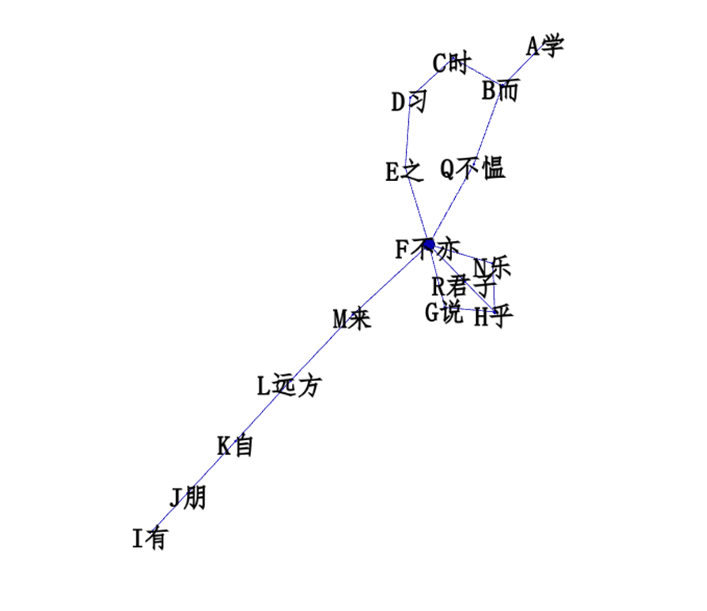
\includegraphics[width=0.5\textwidth]{../example/ccn_example.png}
    \caption{An example of constructing the character co-occurrence network (CCN) from a short text.}
    \label{fig:ccn_example}
    \end{figure}
Figure \ref{fig:ccn_example} illustrates the construction of CCN using a simple example. Given a short text "学而时习之,不亦说乎? 有朋自远方来,不亦乐乎? 人不知自而不愠,不亦君子乎?" (Isn't it a pleasure to study and practice what you have learned? Isn't it delightful to have friends coming from distant quarters? Isn't it characteristic of a noble person to be unaffected when others misunderstand them?), we first extract the unique characters {学,而,时,习,之,不亦,说,乎,有,朋,自,远方,来,不亦,乐,乎,人,不知,而,不愠,不亦,君子,乎} as nodes, and then create edges between adjacent characters, such as (学,而), (而,时), (时,习), (习,之), and so on. The resulting subgraph is then merged into the global CCN.

\subsubsection{Character-Sentence Network (CSN)}
In CSN, two characters are connected by an edge if they co-occur in the same sentence, regardless of their positions. For each sentence in the SS-CC corpus, we create a complete subgraph among all the unique characters in the sentence, and then merge these subgraphs to form the final network. Formally, the CSN can be defined as a graph $G_2=(V_2,E_2)$, where $V_2$ is the set of unique characters and $E_2$ is the set of edges representing sentence-level co-occurrences.
\begin{figure}[htbp]
    \centering
    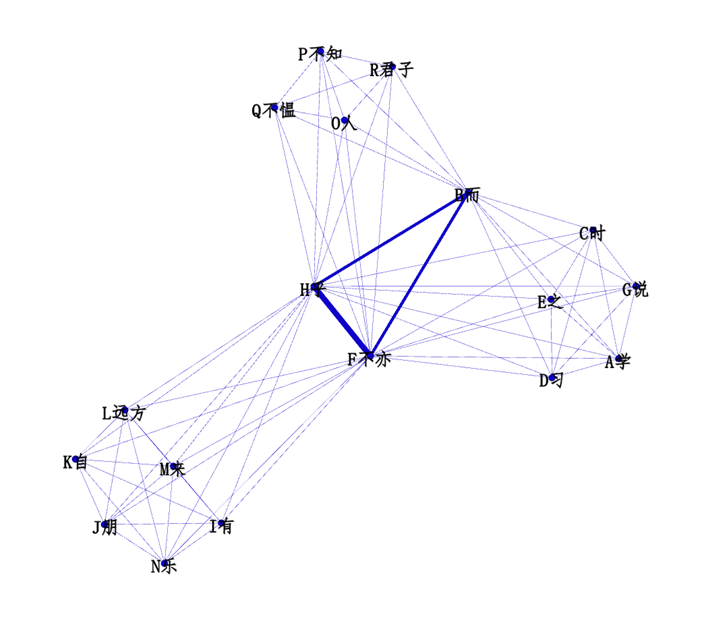
\includegraphics[width=0.5\textwidth]{../example/csn_example.png}
    \caption{An example of constructing the character-sentence network (CSN) from a set of sentences.}
    \label{fig:csn_example}
    \end{figure}
Figure \ref{fig:csn_example} shows an example of constructing CSN from three sentences: "学而时习之,不亦说乎?" , "有朋自远方来,不亦乐乎?" , "人不知自而不愠,不亦君子乎?". For each sentence, a complete subgraph is created among its characters. These subgraphs are then merged to form the global CSN.

The basic statistics of the two networks are summarized in Table \ref{tab:network_stats} and the statistics of corresponding random networks are in Table \ref{tab:control_group_stats}. Due to arithmetic limitations, we are unable to directly compute the clustering coefficients and average shortest path lengths, that is why we use sampling to calculate. In the table following, we uniformly set the sampling ratio to 0.01 and the number of samples to 100. 
\begin{table}[htbp]
    \centering
    \caption{Basic statistics of CCN and CSN}
    \label{tab:network_stats}
    \begin{tabular}{|p{6cm}|c|c|}
        \hline
        \toprule
        Graph & {CCN} & {CSN} \\
        \midrule
        N (Number of nodes) & 156879 & 74837 \\
        E (Number of edges) & 3119616 & 2766801 \\
        $\langle k \rangle$ (Average degree) & 39.77 & 73.96 \\
        C (Clustering coefficient) & 0.022 & 0.046 \\
        L (Average shortest path length) & 2.41 & 2.74 \\
        \bottomrule
    \end{tabular}
\end{table}

\begin{table}[htbp]
    \centering
    \caption{Basic statistics of control group}
    \label{tab:control_group_stats}
    \begin{tabular}{|p{6cm}|c|c|}
        \hline
        \toprule
        Property & {CCN} & {CSN} \\
        \midrule
        N (Number of nodes) & 156879 & 74837 \\
        E (Number of edges) & 3119616 & 2766801 \\
        $\langle k \rangle$ (Average degree) & 39.77 & 73.96 \\
        C (Clustering coefficient) & $2.83 \times 10^{-5}$ & $1.20 \times 10^{-4}$ \\\\
        L (Average shortest path length) & 3.66 & 2.93 \\\\
        \bottomrule
    \end{tabular}
\end{table}
\subsection{Network Analysis Methods}
To analyze the constructed networks, we employ a range of network measures and techniques commonly used in complex network analysis. These include:

\begin{itemize}
    \item Node Strength: Although we analyze unweighted networks, we also introduce and analyze the concept of node strength. If we define the weight of an edge between two nodes as the frequency with which they appear adjacent to each other in the network, then the strength of a node corresponds to its total word frequency.
    \item Degree distribution: The degree distributions show scale-free behavior. Scale-free networks are characterized by a power-law degree distribution, wherein a small number of nodes, called hubs, have a large number of connections. 
    \item Clustering coefficient: The networks' clustering coefficient, which indicates how likely it is for nodes to form clusters. We may determine if the networks have a hierarchical structure—that is, node clusters arranged in a multi-level manner—by examining the correlation between the clustering coefficient and node degree. 
    \item Average shortest path length: To evaluate the efficiency of information transfer and the overall connectivity of the networks, we calculate the average shortest path length. The small-world effect, characterized by small average shortest path length relative to the network size. 
    \item Degree correlations: The average nearest neighbor degree and degree-degree correlations is essential to better understand the degree correlations of the networks. The results of it show whether the networks show assortative or disassortative mixing patterns. 
\end{itemize}
    
The network analysis is performed using Python and popular network analysis libraries NetworkX. As mentioned earlier, due to computational limitations, we employed a sampling approach several times to maintain the overall network properties while reducing the computational burden and improving efficiency.

\section{Models and Results}
This section presents the main findings of our study on the topological properties of CCN and CSN. We focus on the small-world properties, scale-free characteristics, disassortativity and hierarchical structure. These results provide valuable insights into the organizational principles and structural features of Chinese language networks.
\subsection{Small-World Properties}

Compared to a random network with same scale, if a specific network maintains a similar average shortest path length and has a larger clustering coefficient, it is considered to have small world properties \cite{watts1998collective}. Therefore, we investigated the clustering coefficient, and average shortest path length of CCN and CSN to assess their small world properties.
\begin{figure}[htbp]
    \centering
    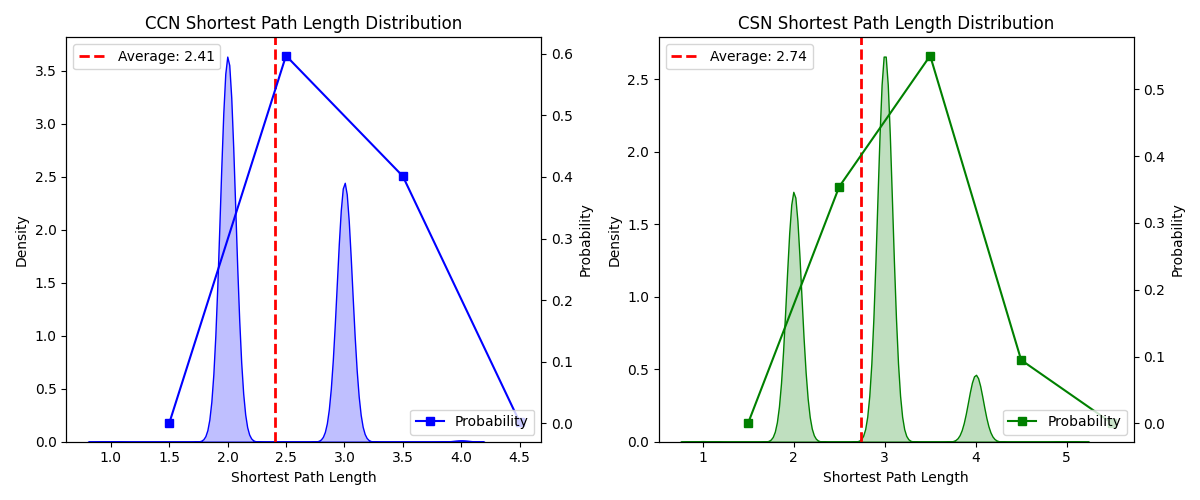
\includegraphics[width=0.8\textwidth]{../analysis/shortest path/shortest path.png}
    \caption{Shortest path length distributions of CCN and CSN. The average shortest path lengths are 2.41 for CCN and 2.74 for CSN.}
    \label{fig:shortest_path}
    \end{figure}
    Compared to an equivalent random network ($C_{\rm rand}=2.83 \times 10^{-5}, L_{\rm rand}=3.66$), CCN has a significantly higher clustering coefficient $C_1=0.022$ and a slightly lower average shortest path length $L_1=2.41$. Similarly, CSN has a higher $C_2=0.046$ and a lower $L_2=2.74$ ($C_{\rm rand}=1.20 \times 10^{-4}, L_{\rm rand}=2.93$). These findings suggest that Classical Chinese lexical networks have strong small-world effects, making information processing and retrieval easier due to their highly connected local clusters and efficient global communication.
\subsection{Scale-Free Characteristics and Matthew Effect}
Many real-world networks exhibit a power-law degree distribution, indicating a scale-free structure \cite{barabasi1999emergence}:
\begin{equation}
P(k) \sim k^{-\gamma}
\end{equation}
\begin{figure}[htbp]
    \centering
    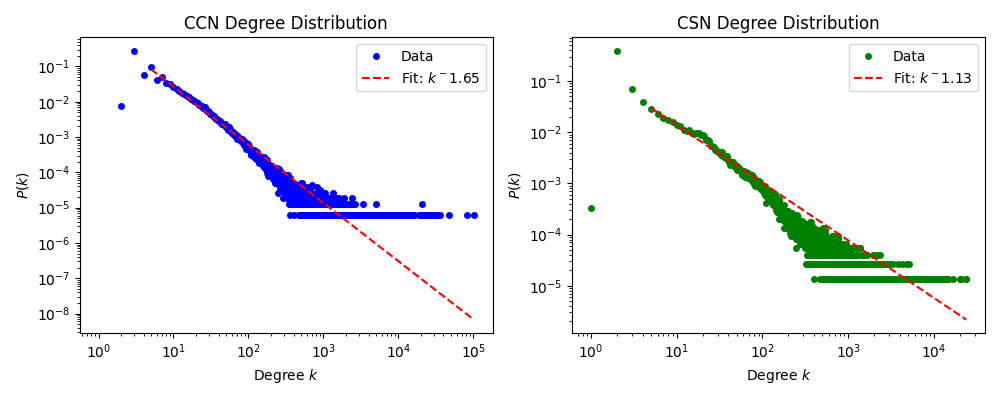
\includegraphics[width=0.8\textwidth]{../analysis/degree distribution/degree distribution.png}
    \caption{Degree distributions of CCN and CSN on a double logarithmic scale. The power-law exponents are 1.65 for CCN and 1.13 for CSN.}
    \label{fig:degree_dist}
    \end{figure}
    The degree distribution $P(k)$ represents the probability that a randomly selected node in the network has degree $k$. Figure \ref{fig:degree_dist} shows the degree distributions of CCN and CSN on a double logarithmic scale. Both networks exhibit power-law tails, indicating a scale-free structure.
    The scale-free nature suggests that a small number of highly connected characters (e.g., function words and common content words, which are usually single characters rather than word combinations in Classical Chinese) play a crucial role in maintaining the connectivity of the Classical Chinese language system.
    To further investigate the relationship between node importance and connection strength, we analyzed the node strength distribution and its correlation with degree.
\begin{figure}[htbp]
    \centering
    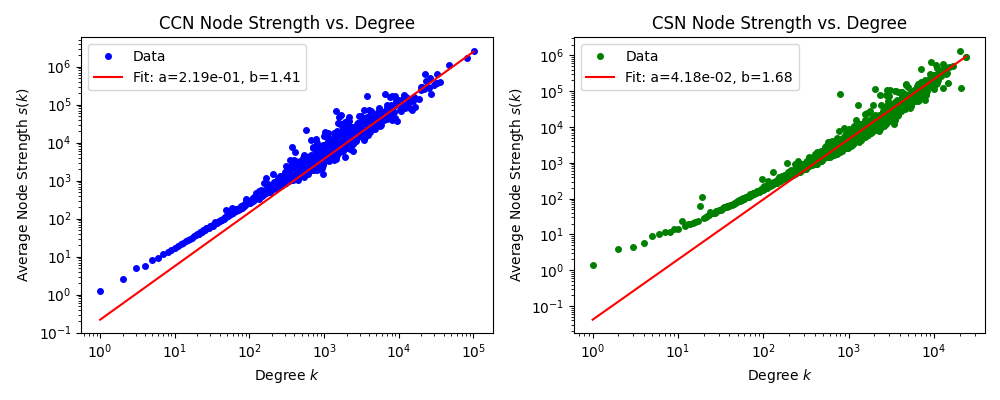
\includegraphics[width=0.8\textwidth]{../analysis/node strength/node strenth.png}
    \caption{Average node strength $s(k)$ vs. degree $k$ for the CCN and CSN networks on a double logarithmic scale. The data is fitted to a power law $s(k) = ak^b$. For CCN, $a=2.19e-01$ and $b=1.41$, indicating a super-linear scaling of node strength with degree. For CSN, $a=4.18e-02$ and $b=1.68$, also showing a super-linear scaling but with a higher exponent compared to CCN.}
    \label{fig:strength_dist}
    \end{figure}
    Figure \ref{fig:strength_dist} shows the node strength distributions of CCN and CSN on a double logarithmic scale. Both networks exhibit heavy-tailed distributions, indicating a highly heterogeneous allocation of connection strengths among nodes. 
    Moreover, we observed a super-linear relationship between node strength $s(k)$ and degree $k$ (Figure \ref{fig:strength_dist}):
    \begin{equation}
    s(k) \sim k^{\alpha}
    \end{equation}
    For CCN, the fitted exponent is $\alpha=1.41$, while for CSN, $\alpha=1.68$. This result suggests that high-degree nodes tend to have disproportionately larger strengths compared to low-degree nodes, pointing to a "Matthew effect" or "rich-get-richer" phenomenon \cite{barabasi1999emergence}.
\subsection{Hierarchical Structure and Disassortativity}
By observing the power-law relationship between the clustering coefficient $C(k)$ and the node degree $k$ \cite{ravasz2003hierarchical}, we can examine whether a complex network possesses a hierarchical structure:
\begin{equation}
C(k) \sim k^{-\beta}
\end{equation}
\begin{figure}[htbp]
    \centering
    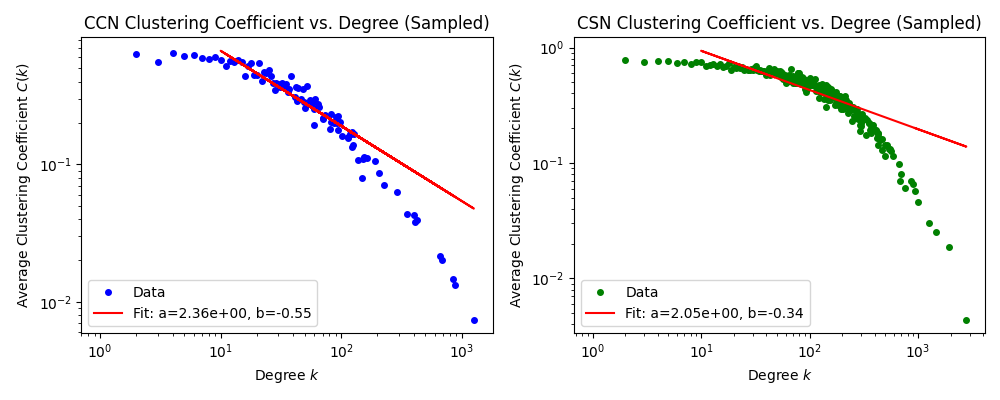
\includegraphics[width=0.8\textwidth]{../analysis/clustering coefficient/clustering coefficient.png}
    \caption{Average clustering coefficient $C(k)$ vs. degree $k$ for the CCN and CSN networks on a double logarithmic scale, using sampled data. The data is fitted to a power law $C(k) = ak^b$. For CCN, $a=2.36e+00$ and $b=-0.55$, indicating a sub-linear decrease of clustering coefficient with degree. For CSN, $a=2.05e+00$ and $b=-0.34$, also showing a sub-linear decrease but with a slower decay compared to CCN.}
    \label{fig:hierarchical}
    \end{figure}
    The hierarchical structures of CCN and CSN reflect the multi-scale, modular organization of the Chinese language system, as shown in Figure \ref{fig:hierarchical}, with $\beta=0.55$ for CCN and $\beta=0.34$ for CSN. There are tightly connected groups at various linguistic unit levels, from radicals to words and phrases.
    In addition, we studied the degree correlations in CSN and CCN to understand the assortativity of the networks. Disassortative mixing is the tendency of high-degree nodes to connect with low-degree nodes, measured by a negative degree correlation coefficient $r$ \cite{newman2002assortative}.
    
\begin{figure}[htbp]
    \centering
    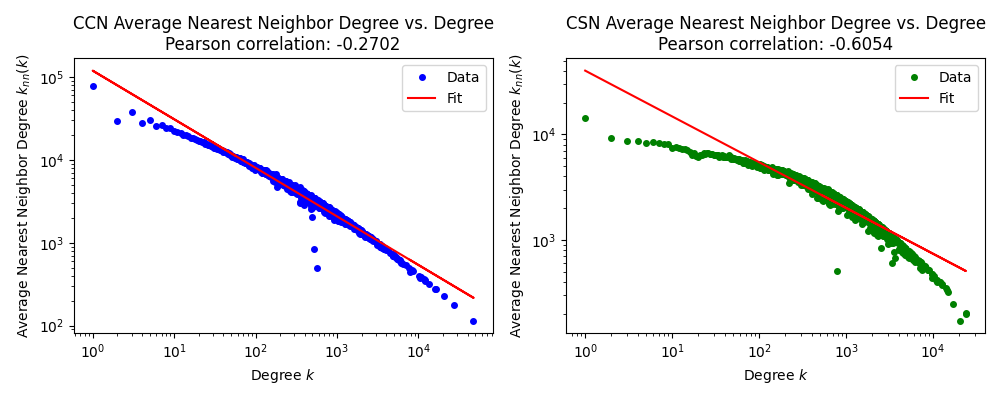
\includegraphics[width=0.8\textwidth]{../analysis/knn/knn.png}
    \caption{Degree correlations in CCN and CSN. The Pearson correlation coefficients are -0.2702 for CCN and -0.6054 for CSN.}
    \label{fig:degree_correlation}
    \end{figure}
    Based on the Pearson correlation coefficient, $r_1=-0.2702$ for CCN and $r_2=-0.6054$ for CSN. Our findings confirm the disassortative nature of CCN and CSN (Figure \ref{fig:degree_correlation}):
    \begin{equation}
    r = \frac{M^{-1}\sum_{i}j_ik_i-[M^{-1}\sum_{i}\frac{1}{2}(j_i+k_i)]^2}{M^{-1}\sum_{i}\frac{1}{2}(j_i^2+k_i^2)-[M^{-1}\sum_{i}\frac{1}{2}(j_i+k_i)]^2}
    \end{equation}
    High-degree function words typically associate with low-degree content words, a phenomenon known as disassortativity, which reflects syntactic and semantic constraints in language organization. Moreover, it may enhance the robustness of the language network against errors and attacks \cite{newman2002assortative}.
\section{Discussion}
Our complex network analysis of the character co-occurrence network (CCN) and the character-sentence network (CSN) constructed from the Scripta Sinica corpus provides novel insights into the organizational principles and statistical regularities of the Classical Chinese language system. The results reveal several non-trivial topological properties, including the scale-free structure, small-world effect, hierarchical organization, and disassortative mixing, which are consistent with the findings of previous studies on modern Chinese and other language networks \cite{sole2010language}. These properties suggest that the Chinese language system, despite its unique features and diachronic evolution, shares some universal characteristics with other human languages, reflecting the common cognitive and communicative constraints in language processing and acquisition.

Comparing our findings with the modern Chinese language networks analyzed in the paper \cite{ZHOU20083039}, we observe many similarities.  Scale-free degree distributions, small-world features, and disassortative mixing patterns are present in both classical and contemporary Chinese networks. The power-law degree distribution of the scale-free structure suggests the existence of strongly connected hub characters or key words in the language system. The small-world effect, which has short average path lengths and substantial local clustering, points to an effective structure for processing and retrieving information. High-degree nodes typically connect with low-degree nodes in disassortative mixing, which is a reflection of the syntactic and semantic limitations in language use. These shared characteristics show how the Chinese language system is both structurally sound and functionally ideal throughout time.

These can be further understood from a language evolution perspective. Grammar, vocabulary, and writing system simplifications and regularizations occurred throughout the Chinese language's transition from the classical to the modern forms \cite{chen1999modern}. But the fundamental organizational ideas—like small-world and scale-free properties—have mostly held true, preserving the harmony between stability and adaptability in language processing and communication.

At the same time, we also observe some differences between the classical and modern Chinese networks. The statistical structure of language networks has changed due to the advent of vernacular Chinese, the standardization of character usage, and the influence of other languages. Based on linguistic theories, we have several speculations about the statistical structure of Classical Chinese texts.

First, due to the concise and highly contextualized nature of Classical Chinese, where characters are more closely related to each other within and across sentences, Classical Chinese networks would be likely to have higher clustering coefficients and shorter average path lengths than their modern counterparts. Second, syntactic rules and semantic categories in Classical Chinese are more rigid compared to the modern vernacular,  implying a stricter separation between function and content characters, so that the disassortative mixing pattern is likely to be more pronounced in the Classical Chinese networks. 

However, not all inferences can be empirically verified through data analysis.

We can demonstrate the more pronounced disassortative mixing pattern in the Classical Chinese networks by comparing the Pearson correlation coefficients: -0.2702 for CCN and -0.6054 for CSN, which are significantly larger in magnitude than -0.0759 for CLN1 and -0.0707 for CLN2.  But we cannot obtain the result that the clustering coefficient is higher and the average path length is shorter in the Classical Chinese networks. 

The indicators that do not align with existing linguistic understanding may have several explanations:

1. Our study is based on a limited corpus of Classical Chinese texts and is not comprehensive. Additionally, statistical result (Total number of characters: 36,762,062, Total number of Chinese characters: 27,868,060, Total number of noise characters: 160,150, Total noise ratio: 0.44\%) shows a significant amount of noise in the texts, which could be a source of bias.

2. Due to technical limitations, we used sampling methods for calculating multiple indicators. Although these methods can yield relatively reliable results, they are still less complete compared to full-scale calculations.

3. During text preprocessing, we were constrained by the lack of a robust NLP model for Classical Chinese. Consequently, we could not create a network that accurately reflects Classical Chinese word segmentation habits, leading to inaccuracies in network construction.
\section{Conclusion}
This study presents a comprehensive complex network analysis of the Classical Chinese language based on the character co-occurrence network (CCN) and the character-sentence network (CSN) constructed from the Scripta Sinica corpus. Our research sheds light on the statistical regularities and organizational principles of the Classical Chinese language system by revealing a variety of non-trivial topological features of the language networks. The following succinctly describes the primary findings of our investigation:

1. The power-law degree distribution of the Classical Chinese language networks indicates a scale-free structure. This suggests that most characters have relatively low degrees, whereas a tiny number of strongly related characters that are essential to the language system exist.

2. The networks display small-world properties, with high local clustering coefficients and short average path lengths. This indicates an efficient organization of the language system for information processing and retrieval, striking a balance between local specialization and global integration.

3. The networks possess a hierarchical modular structure, as evidenced by the power-law relationship between clustering coefficient and degree. This reflects the multi-scale compositional nature of the language system, with characters forming tightly connected clusters at different linguistic levels.

4. The networks show disassortative mixing patterns, where high-degree characters tend to connect with low-degree characters. This property is related to the syntactic and semantic constraints in language organization and may contribute to the robustness and flexibility of the language system.

5. It appears that some organizing principles of human language are universal because the topological characteristics of the Classical Chinese language networks are substantially compatible with those observed in modern Chinese and other language networks. Higher clustering coefficients, shorter path lengths, and more pronounced hierarchical and disassortative structures are some of the major distinctions seen in the Classical Chinese networks, which may be a reflection of the language's distinctive characteristics and evolutionary changes.

These findings offer new insights into the cognitive and communicative mechanisms underpinning language processing and acquisition, as well as the evolutionary and cross-linguistic patterns in human language. They also show how effective complex network theory is at quantitatively characterizing the structure and dynamics of the Chinese language system.


However, it is important to acknowledge the limitations of our study and consider them for future research. First, although extensive, the Scripta Sinica corpus only covers a specific historical period and genre of Classical Chinese literature. The generalizability of our findings to other periods, styles, and registers of the language requires further investigation. Second, our network construction methods, based on character co-occurrence and sentence structure, only capture certain aspects of the language system. Other dimensions of language, such as semantics, pragmatics, morphology, and phonology, are not explicitly represented in the current networks. Third, our analysis focuses primarily on the statistical properties of the language networks, without directly examining the cognitive and social processes underlying language use and evolution. Integrating the network approach with experimental, computational, and historical methods would provide a more comprehensive understanding of the language system.

Despite these limitations, our study opens up new avenues for future research on the complex network analysis of Chinese and other languages. Some promising directions include:

1. Expanding the data sources to include more diverse and representative corpora of Classical and modern Chinese, as well as other languages and dialects, to investigate the universality and specificity of language network properties.

2. Developing more sophisticated network construction methods and analytical tools, such as weighted, directed, and multiplex networks, to capture richer linguistic information and dynamics.

3. To find typological and evolutionary patterns in language networks, conducting methodical comparisons and statistical assessments of network features across various linguistic domains, historical eras, and genres.

4. Combining language acquisition, processing, and change theories and methodologies with network analysis and other linguistic, cognitive, and social theories and methodologies to create a more thorough and explicative framework for comprehending the intricate system of human language.


To conclude, our intricate network analysis of the networks of Classical Chinese languages built from the Scripta Sinica corpus uncovers a wealth of structural features that offer fresh perspectives on the statistical regularities and organizing principles of the language system. Through quantitative characterization and comparison of the structural and functional aspects of human language, the study shows the potential of complex network theory. It also creates new avenues for interdisciplinary research on the cognitive, communicative, and evolutionary bases of language diversity and complexity.
\section*{Acknowledgments}
The data for this study were sourced from the Scripta Sinica database(\url{https://hanchi.ihp.sinica.edu.tw/ihp/hanji.htm}), supported by the Institute of History and Philology, Academia Sinica(\url{https://www1.ihp.sinica.edu.tw/}). We would like to thank @mahavivo(\url{https://github.com/mahavivo/scripta-sinica}) on GitHub and "Daizhige(殆知阁)" for their organization and open sourcing of the documents. We also extend our gratitude to @jiaeyan for providing the Classical Chinese text processing model, Jiayan(甲言)(\url{https://github.com/jiaeyan/Jiayan}).
\section*{Code and Data Availability}
The code and data used in this study are available on GitHub at \url{https://github.com/WhiteMasky/Complex-Network-Analysis-of-Classical-Chinese-Literature}. 

The data preprocessing, network construction, and analysis scripts are provided in the repository, along with the raw and processed data files. The code is written in Python and uses the NetworkX library for network analysis. Everyone is welcome to use and build upon our work for further investigations.
\section*{Ethical Considerations and Broader Impacts}
In this project, we used the Scripta Sinica corpus, which is open source and free for academic research, specifically the sub-corpus of Confucian texts. While Confucianism is representative of Chinese culture, it only reflects a particular aspect of the Chinese language, and the results of our study may not be applicable to other types of Chinese texts. When interpreting and applying our findings, potential limitations and biases in the corpus data, such as variations in text quality, authorship, and genre, should be carefully considered.

Through the use of complex network analysis, the research described in this paper aims to enhance our understanding of the statistical regularities and organizational principles of the Classical Chinese language system. We believe that this study could lead to the development of more effective and efficient techniques for learning, teaching, and processing the Chinese language.

Although the complex network approach provides new insights into the language system, we also acknowledge its limitations and assumptions. The network construction techniques used in our study may not accurately reflect the complexity and diversity of Chinese language use in everyday situations, as they only capture a portion of the character co-occurrence patterns. Therefore, we strongly recommend that future studies replicate and expand on our findings using more representative and diverse datasets of the Chinese language. Additionally, other methodological approaches, such as cross-linguistic comparisons, psycholinguistic experiments, and qualitative analysis, should be used to validate the results.

Regarding broader impacts, we anticipate that our work will stimulate more interdisciplinary studies of Chinese language and culture, thereby bridging the gap between computational techniques and traditional humanities methods. Our complex network framework can be used to model the transmission and evolution of culture, analyze social networks in historical texts, and more. Furthermore, the conclusions of our study may influence the development of more practical tools and technologies for Chinese language processing, including machine translation, information retrieval, and natural language understanding. These technologies can improve accuracy and efficiency by better capturing the structural and semantic patterns of the Chinese language, considering the topological features of language networks.

In the study of language and culture, we caution against blind or over-reliance on computational methods, as they may oversimplify or overlook the complex and diverse aspects of human cognition and communication. It is crucial to strike a balance between quantitative and qualitative methods and to foster ongoing communication and collaboration among researchers with different specializations and backgrounds.

In conclusion, although we believe our research has the potential to improve society in several ways and advance the field of Chinese language studies, we also recognize the risks, biases, and limitations that may be present in our methodology. We welcome further research that expands on and challenges our findings and explores the ethical and societal implications of using complex network analysis to study language and culture.

\bibliographystyle{plain}
\bibliography{../references/references} % 你的 .bib 文件名
\end{document}
